%%% License: Creative Commons Attribution Share Alike 4.0 (see https://creativecommons.org/licenses/by-sa/4.0/)

\documentclass[english,10pt
%,handout
,aspectratio=169
]{beamer}
%%% License: Creative Commons Attribution Share Alike 4.0 (see https://creativecommons.org/licenses/by-sa/4.0/)

\DeclareGraphicsExtensions{.eps, .pdf,.png,.jpg,.mps,}
\usetheme{reMedian}
\usepackage{parskip}
\makeatother

\renewcommand{\baselinestretch}{1.1} 

\usepackage{amsmath, amssymb, amsfonts, amsthm}
\usepackage{enumerate}
%\usepackage{enumitem}
\usepackage{hyperref}
\usepackage{url}
\usepackage{bbm}
\usepackage{color}

\usepackage{tikz}
\usepackage{tikzscale}
\newcommand*\circled[1]{\tikz[baseline=(char.base)]{
		\node[shape=circle,draw, inner sep=-20pt] (char) {#1};}}
\usetikzlibrary{automata,positioning}
\usetikzlibrary{decorations.pathreplacing}
\usepackage{pgfplots}
\usepgfplotslibrary{fillbetween}
\usepackage{graphicx}

\usepackage{setspace}
\thinmuskip=1mu
\medmuskip=1mu 
\thickmuskip=1mu 


\usecolortheme{default}
\usepackage{verbatim}
\usepackage[normalem]{ulem}

\usepackage{apptools}
\AtAppendix{
	\setbeamertemplate{frame numbering}[none]
}
\usepackage{natbib}


% red strikeout
\newcommand\soutred{\bgroup\markoverwith
	{\textcolor{red}{\rule[0.55ex]{2pt}{0.8pt}}}\ULon}



% To use LyX frames from old version:
\def\lyxframeend{} % In case there is a superfluous frame end
\long\def\lyxframe#1{\@lyxframe#1\@lyxframestop}%
\def\@lyxframe{\@ifnextchar<{\@@lyxframe}{\@@lyxframe<*>}}%
\def\@@lyxframe<#1>{\@ifnextchar[{\@@@lyxframe<#1>}{\@@@lyxframe<#1>[]}}
\def\@@@lyxframe<#1>[{\@ifnextchar<{\@@@@@lyxframe<#1>[}{\@@@@lyxframe<#1>[<*>][}}
\def\@@@@@lyxframe<#1>[#2]{\@ifnextchar[{\@@@@lyxframe<#1>[#2]}{\@@@@lyxframe<#1>[#2][]}}
\long\def\@@@@lyxframe<#1>[#2][#3]#4\@lyxframestop#5\lyxframeend{%
	\frame<#1>[#2][#3]{\frametitle{#4}#5}}


\title{Mechanism Design}

\subtitle{0: Introduction}

\author{Egor Starkov}

\date{K{\o}benhavns Unversitet \\
	Fall 2024}


\begin{document}
	\AtBeginSection[]{
		\frame<beamer>{
			\frametitle{This slide deck:}
			\tableofcontents[currentsection,currentsubsection]
	}}
	\frame[plain]{\titlepage}






\section{What is mechanism design?}


\begin{frame}{History of (Micro)Economic Thought (abridged)}
	\centering
	\begin{tabular}{c|c|c}
		\textbf{Question} & \textbf{Answer} & \textbf{Tool}
		\\ \hline
		\pause
		How well do markets work? & \pause Very well! 
			& \begin{tabular}{@{}c@{}}
				Walrasian markets, \\
				First/Second Welfare Theorems
			\end{tabular}
		\\ \hline 
		\pause 
		Why may markets not work? & \pause 
			\begin{tabular}{@{}c@{}}
				Asymmetric information, \\ market power, externalities
			\end{tabular}
			& Game theory
		\\ \hline 
		\pause 
		How to fix the inefficiencies? & \pause We'll see! & Mechanism design!
	\end{tabular}
\end{frame}


\begin{frame}{Not just markets}
	Economics has long sprawled beyond just markets. We, too, will talk about ``markets'' in a very general sense, including, e.g.:
	\pause 
	\begin{itemize}[<+->]
		\item markets for decisions (in groups and societies) and decision rights (in organizations)
		\item markets created by individual interactions (one-on-one, as opposed to many buyers vs many sellers)
		\item markets for partners, roommates, school seats and students
		\item markets without money
		\item markets for information
		\item ...
	\end{itemize}
\end{frame}


%\begin{frame}{What is Game Theory?}
%	\begin{center}
%		Economic agents interact with each other.
%		\pause
%		
%		$\Downarrow$
%		
%		What is the outcome? 
%		\\
%		How is it shaped by environment?
%	\end{center}
%\end{frame}
%
%
%\begin{frame}{What is Mechanism Design?}
%	\begin{center}
%		\pause[2] 
%		How to shape the environment to achieve it?
%		\\
%		(in a strategic setting or a decision problem)
%		
%		$\Uparrow$
%		
%		\pause[1]
%		There is some desirable outcome.
%	\end{center}
%\end{frame}


\begin{frame}{Example 1}
	\begin{columns}
		\begin{column}{0.6\linewidth}
			{\setstretch{1.3}\\
				You want to sell an apartment. What is the best \alert{mechanism} to do so?
				\begin{itemize}
					\item Even setting a \structure{take-it-or-leave-it price} defines some decision problem for a buyer (which price to set then?)
					\pause 
					\item Can \structure{bargaining} perform better than a fixed price?
					\item Should you try to attract more buyers? (How?)
					\item How much info about the apartment do you reveal?
				\end{itemize}
				
				\bigskip 
				Auctions, optimal pricing, and related questions are a large part of mechanism design.
			}
		\end{column}
		\begin{column}{0.4\linewidth}
			\pause[1]
			\includegraphics<handout:0>[width=\linewidth]{pics/M0/8tallet}
		\end{column}
	\end{columns}
\end{frame}


\begin{frame}{Example 2}
	\begin{columns}
		\begin{column}{0.45\linewidth}
			{\setstretch{1.3}\\
				Suppose EU wants to connect its high-speed rail networks. How should the costs be split across countries? 
				\begin{itemize}
					\item Proportional to distance of lines built?
					\item Proportional to costs of lines built?
					\item Proportional to benefits accrued?
					\item ...how to elicit whichever is chosen?
				\end{itemize}
			}
		\end{column}
		\begin{column}{0.55\linewidth}
			\pause[1]
			\includegraphics<handout:0>[width=\linewidth]{pics/M0/rail}
		\end{column}
	\end{columns}
\end{frame}


\begin{frame}{Example 3}
	\begin{columns}
		\begin{column}{0.5\linewidth}
			{\setstretch{1.3}\\
				How to \structure{allocate students to schools}?
				\begin{itemize}
					\item Parents/students have some preferences over schools,
					\item Schools might have priorities over students,
					\item Impossible to respect all preferences.
					\item And we can't use money.
					\item How to organize the application/allocation process to get the best outcome?
				\end{itemize}
			}
		\end{column}
		\begin{column}{0.5\linewidth}
			\pause[1]
			\includegraphics<handout:0>[width=\linewidth]{pics/M0/school}
		\end{column}
	\end{columns}
\end{frame}


%\begin{frame}{What is this course? Problems}
%	We'll be talking a lot about \structure{asymmetric information}. Why?
%	\begin{itemize}
%		\item First Welfare Theorem: competitive markets are efficient and cool and the best.
%		\item So for interesting settings, have to look beyond Walrasian markets
%		\item (asymmetric information, monopoly power, externalities, etc...)
%		\pause\bigskip
%		\item Many \alert{economic problems} deal with asymmetric information:
%		\begin{itemize}
%			\item eliciting a potential buyer's willingness to pay,
%			\item eliciting students' preferences over schools,
%			\item eliciting voters' preferences over candidates,
%			\item etc...
%		\end{itemize}
%	\end{itemize}
%\end{frame}


\begin{frame}{What is this course? Problems}
	\begin{itemize}
		\pause 
		\item \structure{Eliciting hidden information}
		\begin{itemize}
			\item Recall: \alert<1-3>{information asymmetry} is a big source of inefficiencies in markets! Often feeds market power and externalities
			\item Will also look at the complementary question: what's the optimal way to supply information?
		\end{itemize}
		
		\only<1-3>{\visible<3>{\centering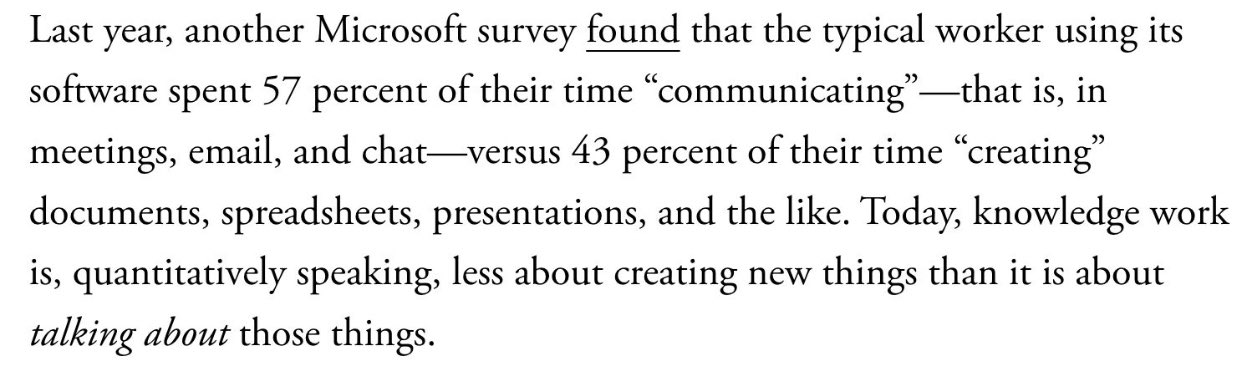
\includegraphics[width=0.82\linewidth]{pics/M0/communicating}}}
		
		\only<4->{
		\item \alert{Hidden action problems} (inducing, monitoring, enforcement)
		\begin{itemize}
			\item We won't look at those, see \textbf{contract theory} course
		\end{itemize}
		
		\item \alert{Aggregating social preferences} / sharing the surplus
		\begin{itemize}
			\item We'll mostly follow the utilitarian approach. See \emph{social choice theory} for more approaches.
			\item Cooperative game theory offers alternative approach to surplus sharing problems.
			\item See also the \textbf{distributive justice} course.
		\end{itemize}
		}
	\end{itemize}
\end{frame}


\begin{frame}{What is this course? Problem-solving skills}
\begin{itemize}
	\pause 
	\item To an extent, this is a course about \alert{formulating problems}:
	\begin{itemize}
		\item \structure<2>{formulating an objective};
		\item \structure<2>{identifying the constraints} that the solution should satisfy.
	\end{itemize}
	
	\pause\bigskip 
	\item Identifying \alert{what constitutes a solution} is an important part of any problem
	\begin{itemize}
		\item What's the solution to $x^2 = 4$? To $a x^2 + bx + c = 0$?
		\pause 
		\item What's the solution to \href{https://www.smbc-comics.com/comic/dilemma-2}{the prisoner's dilemma}? To the lemons market game?
		\pause 
		\item What's the solution to social polarization? To unemployment? To war?
	\end{itemize}
\end{itemize}
\end{frame}


\begin{frame}{What is this course? Methods}
	\begin{itemize}
		\item Most MD problems can be reduced to some \structure{maximization problem}, but a simple Largangian is rarely enough...
		\item (due to high dimensionality of the problems and/or high number of specific constraints)
		\item So we'll also be looking at some \alert{tools and methods} that help solve mechanism design problems.
		\item Can't hope to cover the whole universe of problems, so we'll only look at selected few.
	\end{itemize}
\end{frame}


\begin{frame}{What is this course?}
	What can you expect?
	\begin{itemize}
		\item a crash course on \alert{formalizing problems}
		\item overview of classic results (\structure{problems and solutions}) over past 40 years
		\item a bit from the frontier but not much
		\item and...
		%\item plenty of math! (brace yourselves) (also see math review on absalon)
		%\item intuition and economics behind the models
		%\item models are abstract but are applicable to a \textbf{lot of} areas (industrial organization, political economy, taxation, auctions\ldots{})
		%\item Finally, I hope to give you some practice in economic \textbf{modelling}.
	\end{itemize}
\end{frame}


\begin{frame}
	\begin{columns}
		\begin{column}{0.5\linewidth}
			{\setstretch{1.3}
				...and we need to talk about math
			}
		\end{column}
		\begin{column}{0.48\linewidth}
			\pause[1]
			\href{https://www.smbc-comics.com/comic/what-its-like}{\includegraphics<handout:0>[width=\linewidth]{pics/M0/math2}}
			\vspace{-5ex}
		\end{column}
	\end{columns}
\end{frame}


\begin{frame}{Math}
	\begin{columns}
		\begin{column}{0.8\linewidth}
			{\setstretch{1.3}
				\begin{itemize}
					\item There's a lot of math in this class
					\item Remember: \textbf{you \alert{don't} suck at math!}
					\begin{itemize}
						\item No one is inherently good or bad at math!
					\end{itemize}
					\item Math is just a language you've got to learn
					\item It's difficult, so it's easy to get discouraged
					\begin{itemize}
						\item And the defeatist moods are self-reinforcing
					\end{itemize}
					\item And the only way into it is \alert{practice}
					\begin{itemize}
						\item Believe in yourself and never give up!
					\end{itemize}
				\end{itemize}
				% Possibility:
				% - No one starts good at math: own story 
				% - I self-selected, but I still believe that everyone can do it if they choose to.
				% Why choose to:
				% - Maybe not for own internal logic, but for communication and coordination with other people
				% - Managers have their own "success=leadership*synergy^organization", and it make sense, but economists have to be more precise (in analytics, in policy, in litigation)
			}
		\end{column}
		\begin{column}{0.15\linewidth}
			\pause[1]
			\href{https://www.smbc-comics.com/comic/real-life-3}{\includegraphics<handout:0>[width=\linewidth]{pics/M0/mathskills}}
		\end{column}
	\end{columns}
\end{frame}


\begin{frame}
	\centering
	\includegraphics<handout:0>[width=0.55\linewidth]{pics/M0/howtolearn}
\end{frame}


\begin{frame}
	So you just need to believe in yourself and
	
	\centering
	\href{https://www.youtube.com/watch?v=KxGRhd_iWuE}{\includegraphics<handout:0>[width=0.7\linewidth]{pics/M0/nevergiveup}}
	
	(click this pic every time you feel like you can't do it any more)
\end{frame}


%\begin{frame}{Related courses at KU}
%	\begin{itemize}
%		\item Contract theory, Auctions
%		\item Economics of organization, Corporate Finance, Industrial organization
%		\item Other courses in which applications of mechanism design appear:
%		\begin{itemize}
%			\item Public finance/Taxation
%			\item Political economy
%			\item Monetary
%			\item Labor
%			\item \ldots{}
%		\end{itemize}
%	\end{itemize}
%\end{frame}





\section{Logistics}

\begin{frame}{Hi}
	\begin{itemize}
		\item Egor Starkov
		\item Contact: \texttt{egor.starkov@econ.ku.dk} or absalon inbox
		\item Research interests: information economics, dynamic games, communication
		\item Office: 26.1.13
		\item Office hours: Tue, 14-15
		\item Questions: email/absalon, before/after class
	\end{itemize}
\end{frame}


\begin{frame}{What about you?}
\end{frame}


\begin{frame}{Logistics}
	\begin{itemize}
		\item Weekly lectures (except Fall break -- week \#42)
		\begin{itemize}
			\item Tue, 15:15-18:00, CSS 35.0.12 (but check timetable for room changes)
			\item talk later about what happens in those
		\end{itemize}
		
		%\pause
		%\item Mandatory assignment:
		%\begin{itemize}
		%	\item ``Make your own problem'' -- find an interesting real-world setting and analyze it using the machinery from the class
		%	\item groups of up to 4 are allowed
		%	\item deadline: some time in November?
		%\end{itemize}
		
		\pause
		\item Final exam:
		\begin{itemize}
			\item 12hrs take home (individual, no groups)
			\item Formalize problems; solve them and explain intuition
		\end{itemize}
		
		\pause
		\item Weekly problem sets (ungraded, for practice)
		
		\pause
		\item Research module for PhD students: contact me if you would like to do it
	\end{itemize}
\end{frame}


%\begin{frame}{Covid-specific stuff}
%	\begin{itemize}
%		\item No online streams/recordings are currently planned, back to stone age
%	\end{itemize}
%\end{frame}


\begin{frame}{Workflow}
	\begin{itemize}
		\item Intended workflow: 
		\begin{enumerate}
			\item We start a topic in class (very briefly)
			\item \href{https://www.youtube.com/playlist?list=PL4pUs4P_j1WasI0kO99OgNNd_hJwpct4D}{\uline{You watch video-lectures at home}} during the week (and/or read textbook, slides, papers)
			\item We go through the same material \textbf{very quickly} in class and discuss any questions you have
			\item We solve some problems in class
			\item You have more problems to practice at home
		\end{enumerate}
		\only<1>{Have you noticed the emphasis above? If you don't prepare for lectures, life will be difficult!}
		\pause
		\item Suggestion: organize into study groups. Watch videos in groups. Discuss problems in groups. Let me know by Friday if you want to join a group (assignment on absalon).
		\pause
		\item In class I use whiteboard+slides for ``lecture'' stuff. Slides on absalon include some of the whiteboard parts.
		\begin{itemize}
			\item I'll upload slides in advance, but they might be edited and updated afterwards
		\end{itemize}
		The problems are whiteboard-only; with solutions (mostly) uploaded afterwards.
	\end{itemize}
\end{frame}


\begin{frame}{References: textbooks}
	This course is a compilation of many books, papers, courses; does not follow any single one too closely. Below are some books that might help (see the reading list on Absalon for full references). Note that notation will be different across books and the class!
	\begin{itemize}%[\noitemsep]
		\item \alert{\textbf{Narahari}}: Probably your best bet. Hard to find in print, but you have online access through the library (see Absalon).
		\item \textbf{Diamantaras}: Another good textbook, but seems very hard to find.
		\item \textbf{B\"{o}rgers}: I used this as default in previous years, but it's quite hardcore and hard to follow. (Easy to find though.)
		\item \textbf{MWG}: A microeconomic bible. Very good, very clear, but has the smallest coverage for our course.
		\item \textbf{RS}: Relevant for two lectures on matching. Some material is contained in Narahari and Diamantaras. Nice reference if you are into matching.
	\end{itemize}

\end{frame}


\begin{frame}{References: other}
	\begin{itemize}
		\item I will sometimes refer to individual papers and surveys for results outside of textbooks.
		\item Some of these are completely optional 
		\item Some I expect you to know (but try to explain well enough in the slides).
		\item See the reading list on Absalon for details (will likely be updated during the course).
		%\item survey papers:
		%\begin{description}
		%	\item[B\&V] Bergemann, Dirk, and Juuso Välimäki. ``Dynamic mechanism design: An introduction.'' Journal of Economic Literature 57.2 (2019): 235-74.
		%	\item[B\&M] Bergemann, Dirk, and Stephen Morris. ``Information design: A unified perspective.'' Journal of Economic Literature 57.1 (2019): 44-95. 
		%\end{description}
	\end{itemize}
\end{frame}


%\begin{frame}{References}
%	In the end:
%	\begin{itemize}
	%		\item I suggest getting B{\"o}rgers' textbook. It is not necessary, but might be useful.
	%		\item Diamantaras or MWG are okay alternatives.
	%		\item I do \textbf{not} recommend getting Roth \& Sotomayor textbook unless you are really interested in the topic of matching. Promise the slides will be sufficient for that part of the class.
	%	\end{itemize}
%\end{frame}




\section{First Taste}

\begin{frame}{First taste: Communication problem}
	\begin{block}{Communication problem}
		Can \emph{the designer} elicit \emph{the agent}'s \alert{private information}? How?
	\end{block}
	\begin{itemize}
		\item (``designer'' and ``agent'' are just labels for different players for now)
		\pause 
		\item As usual, \structure{getting to an answer} first requires \alert{understanding the problem}
		\pause
		\item The answer depends on the \structure{nature of the relationship}
		\begin{itemize}
			\item What will the designer do with this knowledge?
			\item How does the agent feel about that?
			\item Let's look at a few examples...
		\end{itemize}
	\end{itemize}
\end{frame}


\begin{frame}{Common interests}
	\begin{exampleblock}{Example 1: Common interests}
		A tourist (principal) is asking a person on the street (agent) which way to the mermaid statue
		\begin{center}
			\begin{tabular}{r | c | c |}
				$(u_P,u_A)$	& $\theta=l$	& $\theta=r$
				\\ \hline 
				$a=L$ 		& $2,1$			& $0,0$
				\\ \hline
				$a=R$		& $0,0$			& $2,1$
				\\ \hline 
			\end{tabular}
		\end{center}
	\end{exampleblock}
	 
	\begin{itemize}
		\item where $\theta\in \{r,l\}$ is the \structure<1>{state of the world} (the correct direction)
		\item $a \in \{L,R\}$ is the \structure<1>{action} the tourist will take (where they will go)
		\item the agent wants to help, knows $\theta$
		\pause \bigskip 
		\item Let's consider a very sophisticated \alert<2>{mechanism} called ``just ask for direction''.
		\pause
		\item The agent would truthfully reveal $\theta$, no reason to lie.
	\end{itemize}
\end{frame}


\begin{frame}{Opposed interests}
	\begin{exampleblock}{Example 2: Opposed interests}
		A judge (principal) is asking a suspect (agent) whether they are guilty of a crime
		\begin{center}
			\begin{tabular}{r | c | c |}
				$(u_P,u_A)$	& $\theta=n$	& $\theta=g$
				\\ \hline 
				$a=N$ 		& $1,2$			& $0,2$
				\\ \hline
				$a=C$		& $0,0$			& $1,0$
				\\ \hline 
			\end{tabular}
		\end{center}
	\end{exampleblock}
	
	\begin{itemize}
		\item where $\theta\in \{g,n\}$ is the \structure<1>{type of the agent} (guilty or not)
		\item $a \in \{C,N\}$ is the judge's \structure<1>{action} (verdict: convict or not)
		\item the agent knows $\theta$, wants $a=N$
		\pause \bigskip 
		\item Just asking would not work: if $\theta=g$, \alert<2>{the agent would lie} and say the state is $\theta=n$.
		\item It is \alert<2>{not possible} to elicit the agent's information
		\item (unless other tools are available)
	\end{itemize}
\end{frame}


\begin{frame}{Partially aligned interests}
	\begin{exampleblock}{Example 3: Partially aligned interests}
		A president (principal) is asking an economic advisor (agent) by how much the spending should be cut.
	\end{exampleblock}
	
	\begin{itemize}
		\item $\theta\in [0,1]$ is the \structure<1>{state of the world} (optimal reduction)
		\item $a \in [0,1]$ is the principal's \structure<1>{action}, wants $a=\theta-b$ for some bias $b<0$
		\item the agent knows $\theta$, wants $a=\theta$
		\pause \bigskip 
		\item \cite{crawford_strategic_1982} show that if $b$ small, there exists a \alert<2>{partially informative} equilibrium($[0,1]$ is partitioned into intervals; agent reveals which interval $\theta$ belongs to)
		\item agent \alert{reveals part} of their private information, but not all of it
	\end{itemize}
\end{frame}




\begin{frame}{Takeaways}
	\begin{itemize}
		\item Agent is willing to reveal their private info if and only if it is in their interest to do so.
		\bigskip 
		\item Can we do \structure<1>{better than ``just asking''}? \pause Turns out, \alert<2>{NO}.
		\item ...But if action is multi-dimensional, can often find partial alignment and \structure<2>{elicit at least some information}.
	\end{itemize}
\end{frame}


\begin{frame}{Partial alignment in multidimensional settings}
	\begin{exampleblock}{Example 4: Multidimensional setting}
		A seller (principal) is asking a potential buyer (agent) about their valuation for the item.
	\end{exampleblock}
	
	\begin{itemize}
		\item $\theta \in [0,1]$ is the \structure<1>{type of the agent} (valuation)
		\item the principal's \structure<1>{action} consists of a price \alert<1>{$p \geq 0$} and a decision \alert<1>{$k \in \{s,r\}$} of whether sell or retain item
		\item the agent knows $\theta$, wants $k=s$ if $p$ low and $k=r$ otherwise
		\item the principal wants the opposite
		\pause \bigskip 
		\item Despite opposing interests, trade \structure{can} occur (e.g., via the seller announcing some price at which they're willing to sell, and the buyer choosing whether to accept it or not).
	\end{itemize}
\end{frame}


\begin{frame}{Takeaways}
	\begin{itemize}
		\item Agent is willing to reveal their private info if and only if it is in their interest to do so.
		\bigskip 
		\item Can we do better than ``just asking''? Turns out, NO.
		\item ...But if action is multi-dimensional, can often find partial alignment and elicit at least some information.
	\end{itemize}
\end{frame}


\begin{frame}{For next week}
	\begin{enumerate}
		\item Split into study groups (if you are looking for a group: respond to an assignment on absalon by Friday or email me)
		\item Have a look at math review notes on absalon
		\item Watch lectures 2.1 (`What is a mechanism?') and 2.2 (`Dominant strategy implementation') \href{https://www.youtube.com/playlist?list=PL4pUs4P_j1WasI0kO99OgNNd_hJwpct4D}{\uline{on youtube}}.
		\begin{itemize}
			\item Or read Narahari ch.14-16
		\end{itemize}
	\end{enumerate}
\end{frame}


\appendix
\begin{frame}[allowframebreaks]{References}
	\bibliography{teaching}
	\bibliographystyle{abbrvnat}
\end{frame}


\end{document}